\documentclass[a4paper,14pt]{extreport} % формат документа

\usepackage{amsmath}
\usepackage{cmap} % поиск в ПДФ
\usepackage[T2A]{fontenc} % кодировка
\usepackage[utf8]{inputenc} % кодировка исходного текста
\usepackage[english,russian]{babel} % локализация и переносы
\usepackage[left = 2cm, right = 1cm, top = 2cm, bottom = 2 cm]{geometry} % поля
\usepackage{listings}
\usepackage{graphicx} % для вставки рисунков
\usepackage{amsmath}
\usepackage{float}
\usepackage{multirow}
\graphicspath{{pictures/}}
\DeclareGraphicsExtensions{.pdf,.png,.jpg}
\newcommand{\anonsection}[1]{\section*{#1}\addcontentsline{toc}{section}{#1}}

\lstset{ %
	language=C,                % Язык программирования 
	numbers=left,                   % С какой стороны нумеровать          
	frame=single,                    % Добавить рамку
	basicstyle=\small,
    escapebegin=\begin{russian}\commentfont,
    escapeend=\end{russian},
    literate={Ö}{{\"O}}1
    {Ä}{{\"A}}1
    {Ü}{{\"U}}1
    {ß}{{\ss}}1
    {ü}{{\"u}}1
    {ä}{{\"a}}1
    {ö}{{\"o}}1
    {~}{{\textasciitilde}}1
    {а}{{\selectfont\char224}}1
    {б}{{\selectfont\char225}}1
    {в}{{\selectfont\char226}}1
    {г}{{\selectfont\char227}}1
    {д}{{\selectfont\char228}}1
    {е}{{\selectfont\char229}}1
    {ё}{{\"e}}1
    {ж}{{\selectfont\char230}}1
    {з}{{\selectfont\char231}}1
    {и}{{\selectfont\char232}}1
    {й}{{\selectfont\char233}}1
    {к}{{\selectfont\char234}}1
    {л}{{\selectfont\char235}}1
    {м}{{\selectfont\char236}}1
    {н}{{\selectfont\char237}}1
    {о}{{\selectfont\char238}}1
    {п}{{\selectfont\char239}}1
    {р}{{\selectfont\char240}}1
    {с}{{\selectfont\char241}}1
    {т}{{\selectfont\char242}}1
    {у}{{\selectfont\char243}}1
    {ф}{{\selectfont\char244}}1
    {х}{{\selectfont\char245}}1
    {ц}{{\selectfont\char246}}1
    {ч}{{\selectfont\char247}}1
    {ш}{{\selectfont\char248}}1
    {щ}{{\selectfont\char249}}1
    {ъ}{{\selectfont\char250}}1
    {ы}{{\selectfont\char251}}1
    {ь}{{\selectfont\char252}}1
    {э}{{\selectfont\char253}}1
    {ю}{{\selectfont\char254}}1
    {я}{{\selectfont\char255}}1
    {А}{{\selectfont\char192}}1
    {Б}{{\selectfont\char193}}1
    {В}{{\selectfont\char194}}1
    {Г}{{\selectfont\char195}}1
    {Д}{{\selectfont\char196}}1
    {Е}{{\selectfont\char197}}1
    {Ё}{{\"E}}1
    {Ж}{{\selectfont\char198}}1
    {З}{{\selectfont\char199}}1
    {И}{{\selectfont\char200}}1
    {Й}{{\selectfont\char201}}1
    {К}{{\selectfont\char202}}1
    {Л}{{\selectfont\char203}}1
    {М}{{\selectfont\char204}}1
    {Н}{{\selectfont\char205}}1
    {О}{{\selectfont\char206}}1
    {П}{{\selectfont\char207}}1
    {Р}{{\selectfont\char208}}1
    {С}{{\selectfont\char209}}1
    {Т}{{\selectfont\char210}}1
    {У}{{\selectfont\char211}}1
    {Ф}{{\selectfont\char212}}1
    {Х}{{\selectfont\char213}}1
    {Ц}{{\selectfont\char214}}1
    {Ч}{{\selectfont\char215}}1
    {Ш}{{\selectfont\char216}}1
    {Щ}{{\selectfont\char217}}1
    {Ъ}{{\selectfont\char218}}1
    {Ы}{{\selectfont\char219}}1
    {Ь}{{\selectfont\char220}}1
    {Э}{{\selectfont\char221}}1
    {Ю}{{\selectfont\char222}}1
    {Я}{{\selectfont\char223}}1
    {і}{{\selectfont\char105}}1
    {ї}{{\selectfont\char168}}1
    {є}{{\selectfont\char185}}1
    {ґ}{{\selectfont\char160}}1
    {І}{{\selectfont\char73}}1
    {Ї}{{\selectfont\char136}}1
    {Є}{{\selectfont\char153}}1
    {Ґ}{{\selectfont\char128}}1
}

\begin{document}
\begin{titlepage}

    \begin{table}[H]
        \centering
        \footnotesize
        \begin{tabular}{cc}
            \multirow{8}{*}{
\includegraphics[scale=0.35]{bmstu.jpg}}
            & \\
            & \\
            & \textbf{Министерство науки и высшего образования Российской Федерации} \\
            & \textbf{Федеральное государственное бюджетное образовательное учреждение} \\
            & \textbf{высшего образования} \\
            & \textbf{<<Московский государственный технический} \\
            & \textbf{университет имени Н.Э. Баумана>>} \\
            & \textbf{(МГТУ им. Н.Э. Баумана)} \\
        \end{tabular}
    \end{table}

    \vspace{-2.5cm}

    \begin{flushleft}
        \rule[-1cm]{\textwidth}{3pt}
        \rule{\textwidth}{1pt}
    \end{flushleft}

    \begin{flushleft}
        \small
        ФАКУЛЬТЕТ
        \underline{<<Информатика и системы управления>>\ \ \ \ \ \ \ 
        \ \ \ \ \ \ \ \ \ \ \ \ \ \ \ \ \ \ \ \ \ \ \ \ \ \ \ \ \ \ \ 
    \ \ \ \ \ \ \ \ \ \ \ \ \ \ \ } \\
        КАФЕДРА
        \underline{<<Программное обеспечение ЭВМ и
        информационные технологии>>
        \ \ \ \ \ \ \ \ \ \ \ \ \ \ \ \ \ \ \ \ }
    \end{flushleft}

    \vspace{2cm}

    \begin{center}
        \textbf{Лабораторная работа № 4} \\
        \vspace{0.5cm}
    \end{center}

    \vspace{4cm}

    \begin{flushleft}
        \begin{tabular}{ll}
            \textbf{Дисциплина} & Операционные системы.  \\
            \textbf{Тема} & Виртуальная файловая система /proc.  \\
            \\
            \textbf{Студент} & Сиденко А.Г. \\
            \textbf{Группа} & ИУ7-63Б \\
            \textbf{Оценка (баллы)} & \\
            \textbf{Преподаватель} & Рязанова Н.Ю.   \\
        \end{tabular}
    \end{flushleft}

    \vspace{4cm}

   \begin{center}
        Москва, 2020 г.
    \end{center}

\end{titlepage}

\subsubsection{Часть 1}

\hfill

\textbf{Задание: } Используя виртуальную файловую систему proc вывести информацию об окружении процесса, информацию, характеризующую состояние процесса, содержание директории fd и файла cmdline.

\begin{lstlisting}[caption=Часть 1. ]
#include <sys/stat.h>
#include <dirent.h>
#include <stdio.h>
#include <stdlib.h>
#include <string.h>
#include <errno.h>
#include <unistd.h>

#define BUF_SIZE 0x1000

// Вывод содержимого файла ENVIRON
void readEnviron()
{
  char buf[BUF_SIZE];
  int len, i;
  FILE *f = fopen("/proc/self/environ", "r");
  if (f == NULL)
  {
    printf("%s", strerror(errno));
    exit(errno);
  }

  while ((len = fread(buf, 1, BUF_SIZE, f)) > 0)
  {
    for (i = 0; i < len; i++)
      if (buf[i] == 0)
        buf[i] = 10; // код 10, перевод строки
    buf[len] = 0;
    printf("%s", buf);
  }

  fclose(f);
}

// Вывод содержимого файла STAT, CMDLINE
void readFile(char *path)
{
  char buf[BUF_SIZE];
  FILE *f = fopen(path, "r");
  if (f == NULL)
  {
    printf("%s", strerror(errno));
    exit(errno);
  }

  fread(buf, 1, BUF_SIZE, f);
  char *pch = strtok(buf, " "); // поиск разделителей в файле

  while (pch != NULL)
  {
    printf("%s\n", pch);
    pch = strtok(NULL, " "); // продолжение сканирование с того места,
                             // где был остановлен предыдущий 
                             // успешный вызов функции
  }

  fclose(f);
}

// Вывод содержимого директории FD
void contentDir()
{
  struct dirent *dirp;
  DIR *dp;
  char str[BUF_SIZE];
  char path[BUF_SIZE];

  if ((dp = opendir("/proc/self/fd/")) == NULL)
  {
    printf("%s", strerror(errno));
    exit(errno);
  }

  while ((dirp = readdir(dp)) != NULL)
  {
    // Пропуск каталогов . и ..
    if ((strcmp(dirp->d_name, ".")!=0)&&(strcmp(dirp->d_name, "..")!=0))
    {
      sprintf(path, "%s%s", "/proc/self/fd/", dirp->d_name);
      readlink(path, str, BUF_SIZE); // Считывает значение 
      				     // символьной ссылки
      printf("%s -> %s\n", dirp->d_name, str);
    }
  }
   
  if (closedir(dp) < 0)
  {
    printf("%s", strerror(errno));
    exit(errno);
  }
}

int main(int argc, char *argv[])
{
  if (argc != 2)
  {
    printf("Использование: ./output.exe <stat/environ/fd/cmdline>\n");
    return 1;
  }

  if (strcmp("environ", argv[1]) == 0)
    readEnviron();
  else if (strcmp("stat", argv[1]) == 0)
    readFile("/proc/self/stat");
  else if (strcmp("fd", argv[1]) == 0)
    contentDir("/proc/self/fd/");
  else if (strcmp("cmdline", argv[1]) == 0)
    readFile("/proc/self/cmdline");
  else
    printf("Использование: ./output.exe <stat/environ/fd/cmdline>\n");

  return 0;
}
\end{lstlisting}

\begin{enumerate}
\item Список окружения процесса (environ):

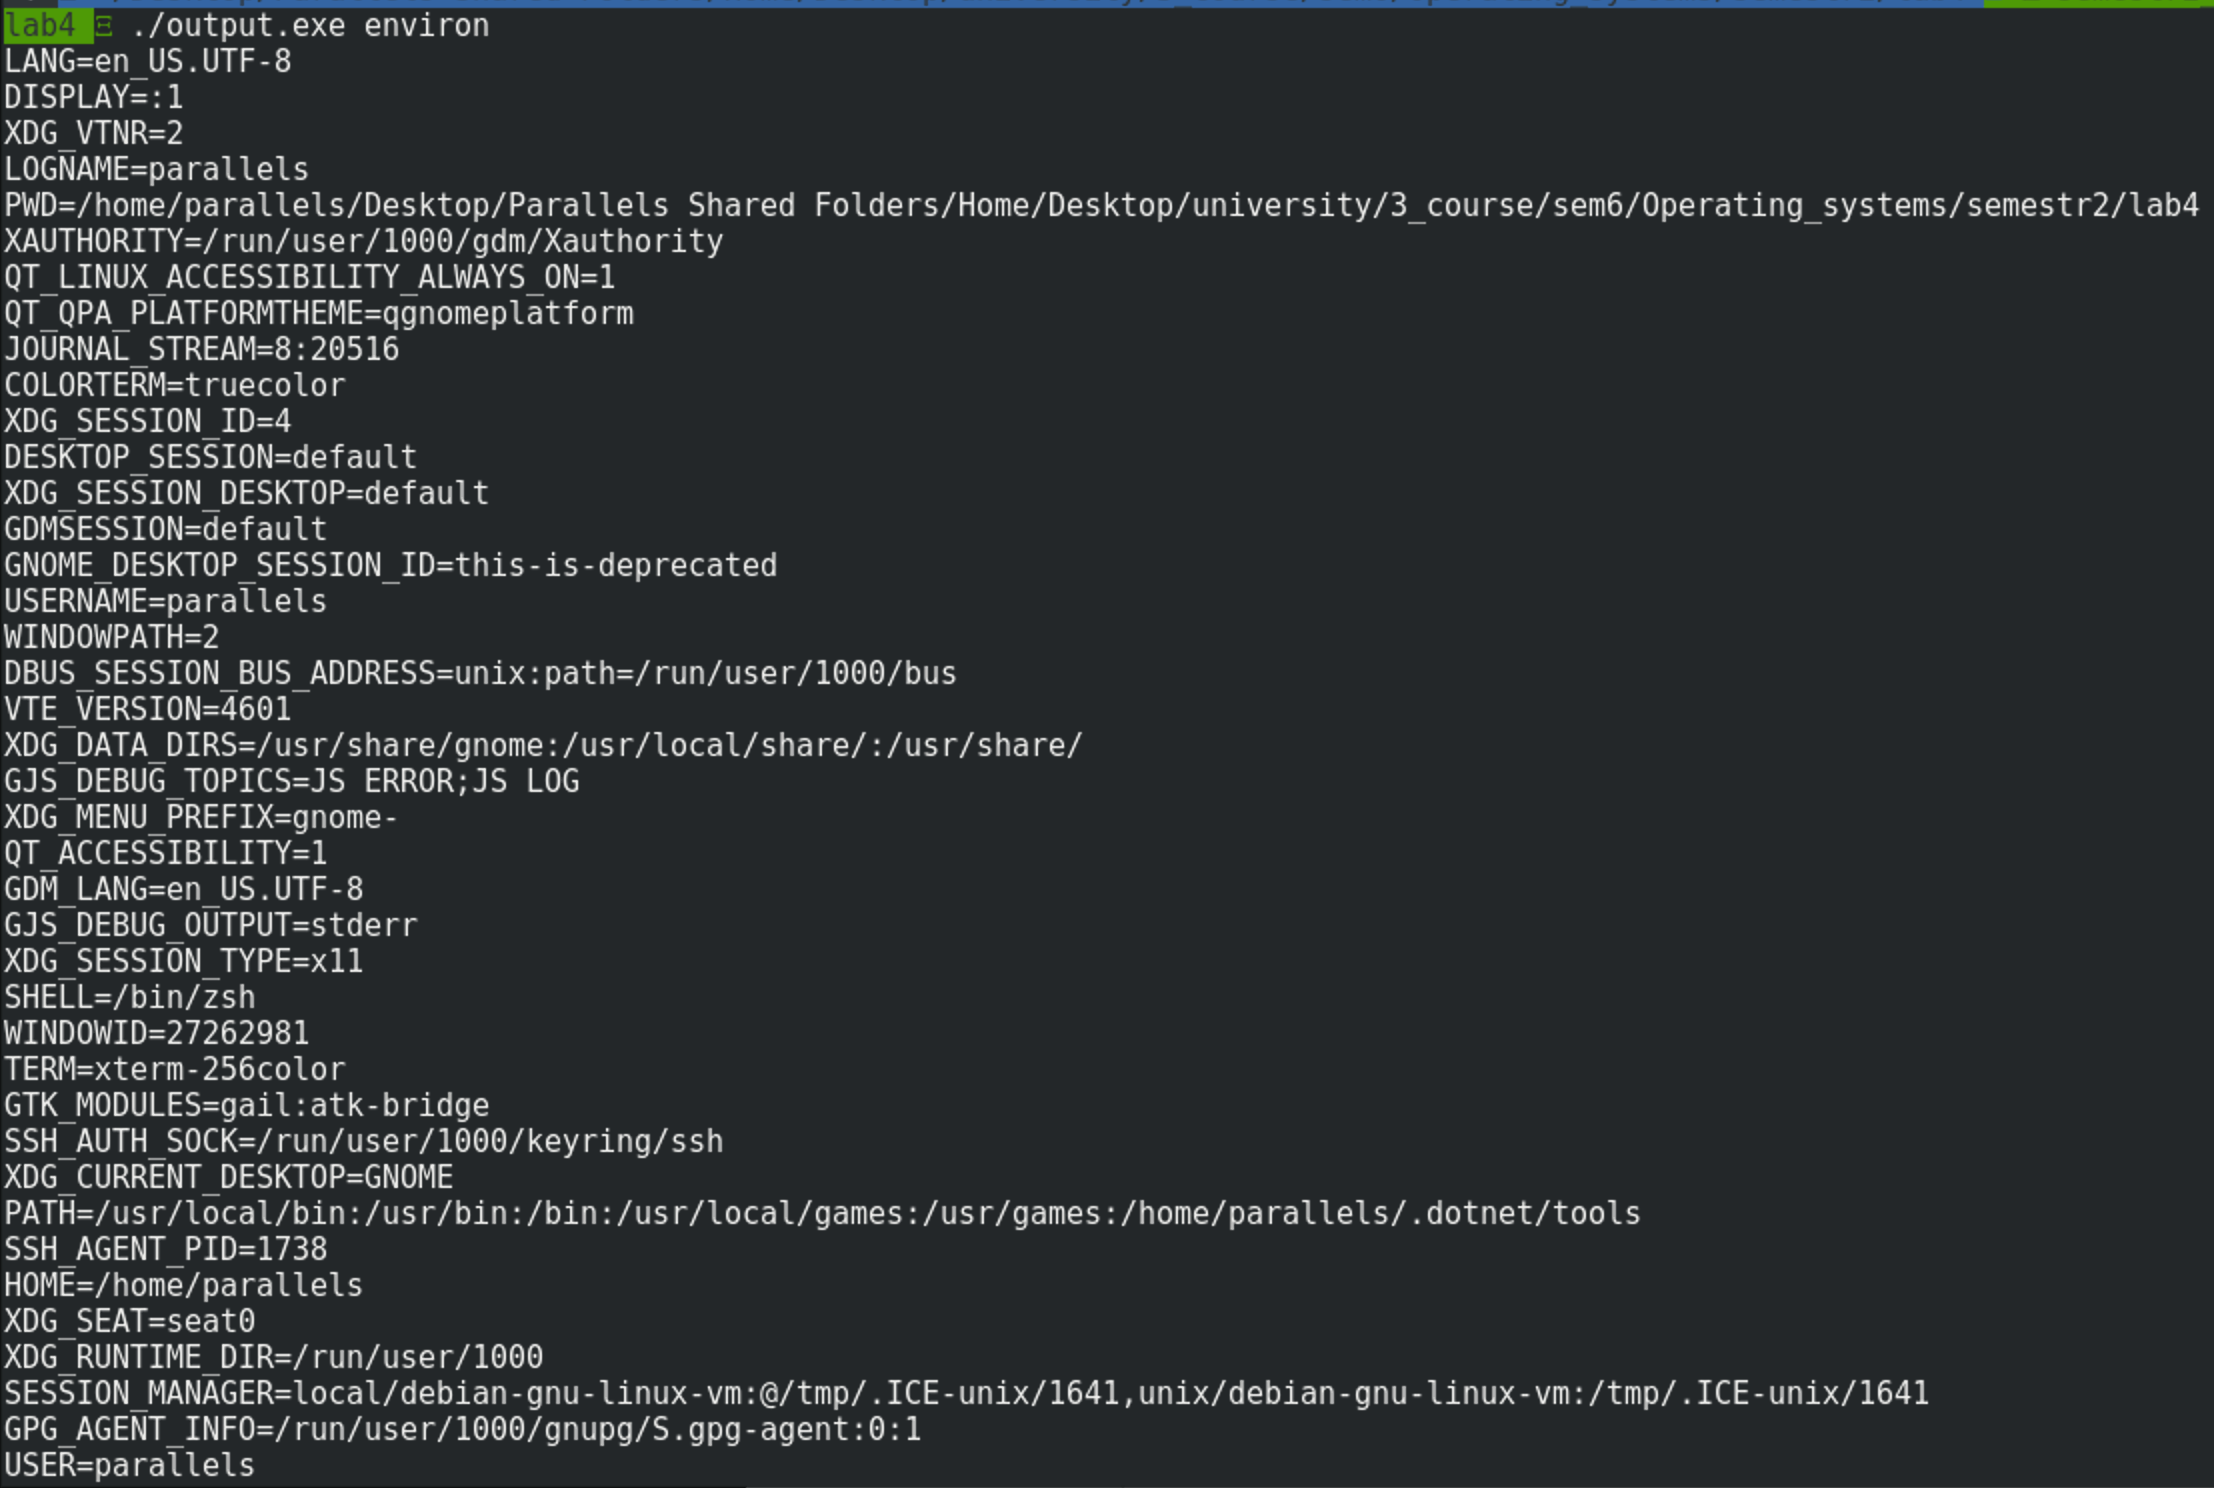
\includegraphics[scale=0.45]{images/environ}

\item Информация о процессе (stat):

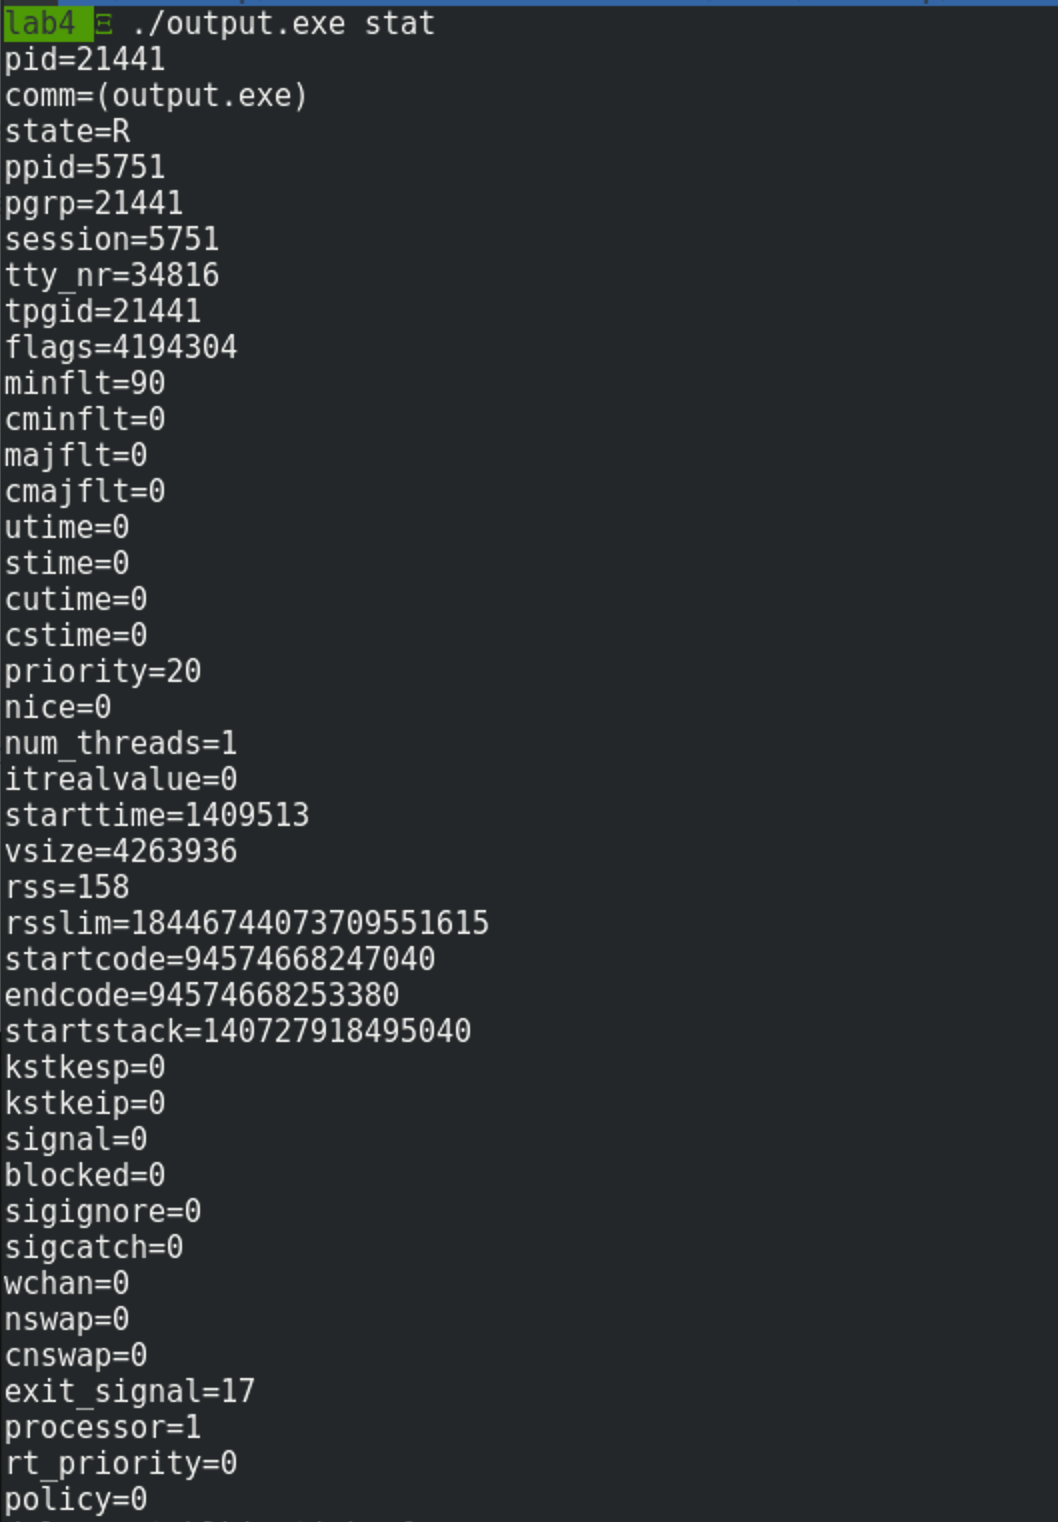
\includegraphics[scale=0.45]{images/stat}

\item Директория процесса (cmdline):

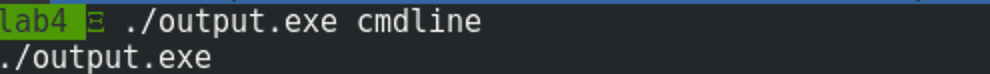
\includegraphics[scale=0.45]{images/cmdline}

\item Ссылки на файлы, которые «открыл» процесс (fd):

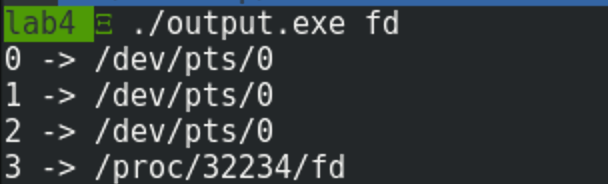
\includegraphics[scale=0.45]{images/fd}

\end{enumerate}

\newpage

\subsubsection{Часть 2}

\hfill

\textbf{Задание: } Написать загружаемый модуль ядра, создать файл в файловой системе proc, sysmlink, subdir. Используя соответствующие функции передать данные из пространства пользователя в пространство ядра (введенные данные вывести в файл ядра) и из пространства ядра в пространство пользователя. Продемонстрировать это.

\begin{lstlisting}[caption=Часть 2. ]
#include <linux/module.h>
#include <linux/kernel.h>
#include <linux/proc_fs.h>
#include <linux/string.h>
#include <linux/vmalloc.h>
#include <linux/fs.h>
#include <asm/uaccess.h>

MODULE_LICENSE("GPL");
MODULE_AUTHOR("Sidenko");
MODULE_DESCRIPTION("Lab4");

static struct proc_dir_entry *proc_entry, *dir, *symlink;
static char* buffer; // Хранилище 'фортунок'
int buffer_index, next_fortune; // Индексы для записи и вывода

ssize_t fortune_write(struct file *filp, const char __user *buf, 
					size_t len, loff_t *offp)
{
  int space_available = (PAGE_SIZE - buffer_index) + 1;

  // Хватит ли места для размещения
  if (len > space_available)
    return -ENOSPC;

  // Копирование строки
  if (copy_from_user(&buffer[buffer_index], buf, len))
    return -EFAULT;

  buffer_index += len;
  buffer[buffer_index - 1] = '\n';

  return len;
}

ssize_t fortune_read(struct file *filp, char __user *buf, size_t count, 
						loff_t *offp)
{
  int len;
  if (*offp > 0)
    return 0;

  // Перевод индекса на первый элемент
  if (next_fortune >= buffer_index)
    next_fortune = 0;

  len = copy_to_user(buf, &buffer[next_fortune], count);
  next_fortune += len;
  *offp += len;

  return len;
}

struct file_operations fileops =
{
  .read = fortune_read,
  .write = fortune_write
};

int fortune_module_init(void)
{
  buffer = (char *)vmalloc(PAGE_SIZE);
  if (!buffer)
  {
    printk(KERN_INFO "fortune: No memory for create buffer\n");
    return -ENOMEM;
  }
  memset(buffer, 0, PAGE_SIZE);

  proc_entry = proc_create("fortune", 0666, NULL, &fileops);
  if (proc_entry == NULL)
  {
    vfree(buffer);
    printk(KERN_INFO "fortune: Couldn't create proc entry\n");
    return -ENOMEM;
  }

  dir = proc_mkdir("fortune_dir", NULL);
  symlink = proc_symlink("fortune_symlink", NULL, "/proc/fortune_dir");
  if ((dir == NULL) || (symlink == NULL))
  {
    vfree(buffer);
    printk(KERN_INFO "fortune: Couldn't create proc dir, symlink\n");
    return -ENOMEM;
  }

  buffer_index = 0;
  next_fortune = 0;

  printk(KERN_INFO "fortune: Module loaded.\n");
  return 0;
}

void fortune_module_exit(void)
{
  remove_proc_entry("fortune", NULL);
  remove_proc_entry("fortune_symlink", NULL);
  remove_proc_entry("fortune_dir", NULL);
  vfree(buffer);
  printk(KERN_INFO "fortune: Module unloaded.\n");
}

module_init(fortune_module_init);
module_exit(fortune_module_exit);
\end{lstlisting}

\begin{enumerate}
\item Собираем, загружаем модуль ядра, проверяем создание файла, директории, символьной ссылки:

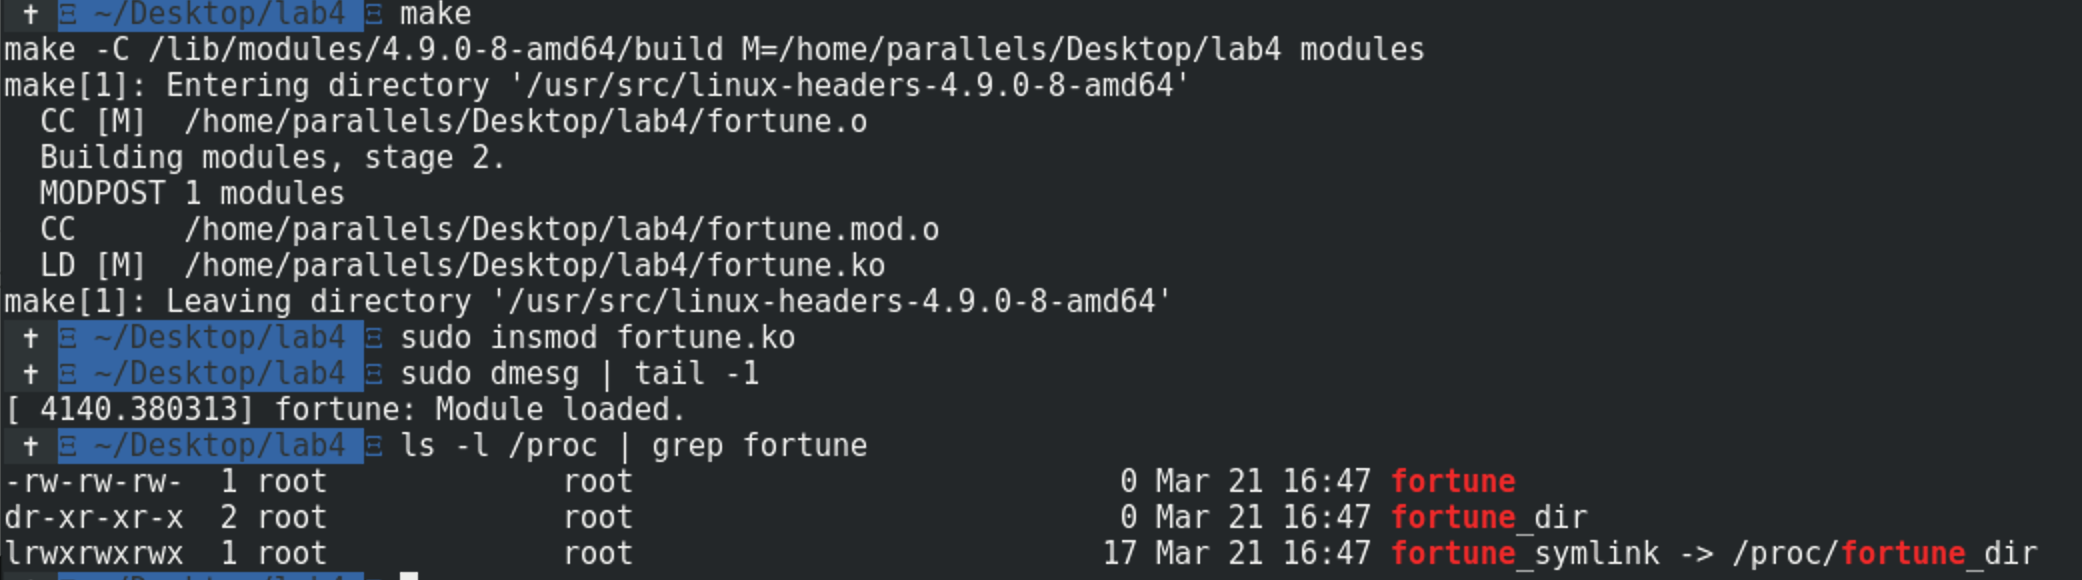
\includegraphics[scale=0.45]{images/insmod}

\item Посылка и считывание данных:

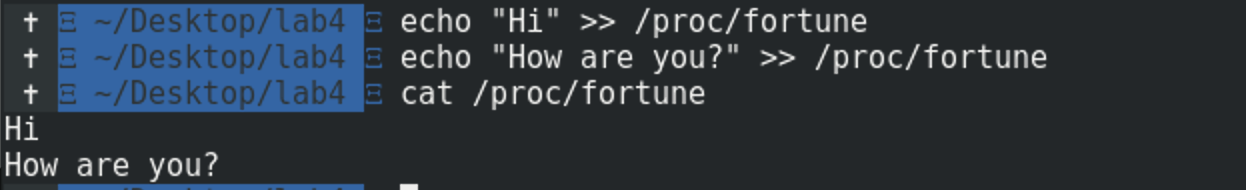
\includegraphics[scale=0.45]{images/cat}

\item Выгружаем модуль:

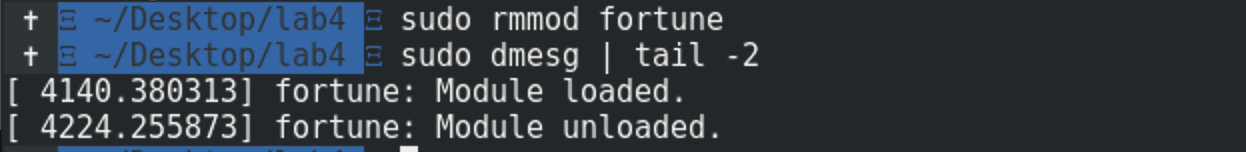
\includegraphics[scale=0.45]{images/rmmod}

\end{enumerate}

\end{document}